\documentclass[a4paper,10pt,notitlepage]{article}
\usepackage{ctex,geometry,graphicx,tikz,setspace,paralist,fancyhdr,caption}
\geometry{
	left=1.5cm,
	right=1.5cm,
	top=1.4cm,
	bottom=2cm,}
\newcommand{\rec}{
	\begin{tikzpicture}[remember picture,overlay]
		% 绘制边框
		\draw[line width=1.2pt] ([xshift=0.5cm,yshift=0.5cm] current page.south west) rectangle ([xshift=-0.5cm,yshift=-0.8cm] current page.north east);
	\end{tikzpicture}
	
}
\pagestyle{fancy}
\fancyhf{}
\fancyhead[C]{\rec}  % 在页眉中绘制图形
\fancyhead[L]{附录}
\fancyhead[R]{实验四 \quad 射极跟随器}
\fancyfoot[C]{\thepage}
\begin{document}
	\large
	\onehalfspacing
	\begin{figure}[h]
		\raggedright
		\includegraphics{../1.png}
	\end{figure}
	\centering
	{\Huge\textbf{模电实验报告}\par}
	\vspace{0.2cm}
	{\huge{实验内容:射极跟随器}\par}
	\raggedright
	\vspace{0.3cm}
	\begin{centering}
		{\large 院系:电子与信息工程学院\hfill 学号:22309080\hfill 审批:\hspace{2cm} \par
			专业:通信工程\hfill 实验人:梁倍铭\hfill 日期:2023年11月9日 \par}
	\end{centering}
	\vspace{0.3cm}
	\section*{一、直流工作点的调整}
	\begin{figure}[h]
		\raggedright
		\begin{minipage}{0.3\textwidth}
			\centering
			\includegraphics[width=\textwidth]{1.png}
			\caption*{仿真电路图}
		\end{minipage}
		\qquad
		\begin{minipage}{0.28\textwidth}
			\centering
			\includegraphics[width=\textwidth]{2.png}
			\caption*{仿真波形}
		\end{minipage}
		\qquad
		\begin{minipage}{0.28\textwidth}
			\centering
			
\includegraphics[width=\textwidth]{3.png}
			\caption*{仿真结果}
		\end{minipage}
	\end{figure}
	\begin{figure}[h]
		\centering
			\begin{tabular}{|c|c|c|c|c|}
			\hline
			& $V_e(V)$ & $V_b(V)$ & $V_c(V)$ & $I_c=V_e/R_e$ \\
			\hline
			仿真 & 6.02531 & 6.68479 & 6.08098 & 3.01mV \\
			\hline
			实验 & \quad & \quad & \qquad & \quad  \\
			\hline
		\end{tabular}
		\caption*{表4-1 }
	\end{figure}
	\newpage
	\section*{二、测量电压放大倍数}
		\begin{figure}[h]
		\centering
		\begin{tabular}{|c|c|c|c|}
			\hline
			& $V_i(V)$ & $U_o(V)$ & $A_v=U_o/U_i$ \\
			\hline
			仿真 & 2.4 & 2.28 &  0.95 \\
			\hline
			实验 & \quad & \quad & \qquad  \\
			\hline
		\end{tabular}
		\caption*{表4-2 }
	\end{figure}
		\begin{figure}[h]
		\raggedright
		\begin{minipage}{0.3\textwidth}
			\centering
			
\includegraphics[width=\textwidth]{4.png}
			\caption*{仿真电路图}
		\end{minipage}
		\qquad
		\begin{minipage}{0.28\textwidth}
			\centering
			
\includegraphics[width=\textwidth]{5.png}
			\caption*{仿真波形}
		\end{minipage}
		\qquad
		\begin{minipage}{0.28\textwidth}
			\centering
			\includegraphics[width=\textwidth]{5-1.png}
			\caption*{仿真结果}
		\end{minipage}
	\end{figure}
	\section*{三、测量输出电阻}
	\begin{figure}[h]
		\raggedright
		\begin{minipage}{0.3\textwidth}
			\centering
			\includegraphics[width=\textwidth]{6.png}
			\caption*{仿真电路图}
		\end{minipage}
		\qquad
		\begin{minipage}{0.28\textwidth}
			\centering
			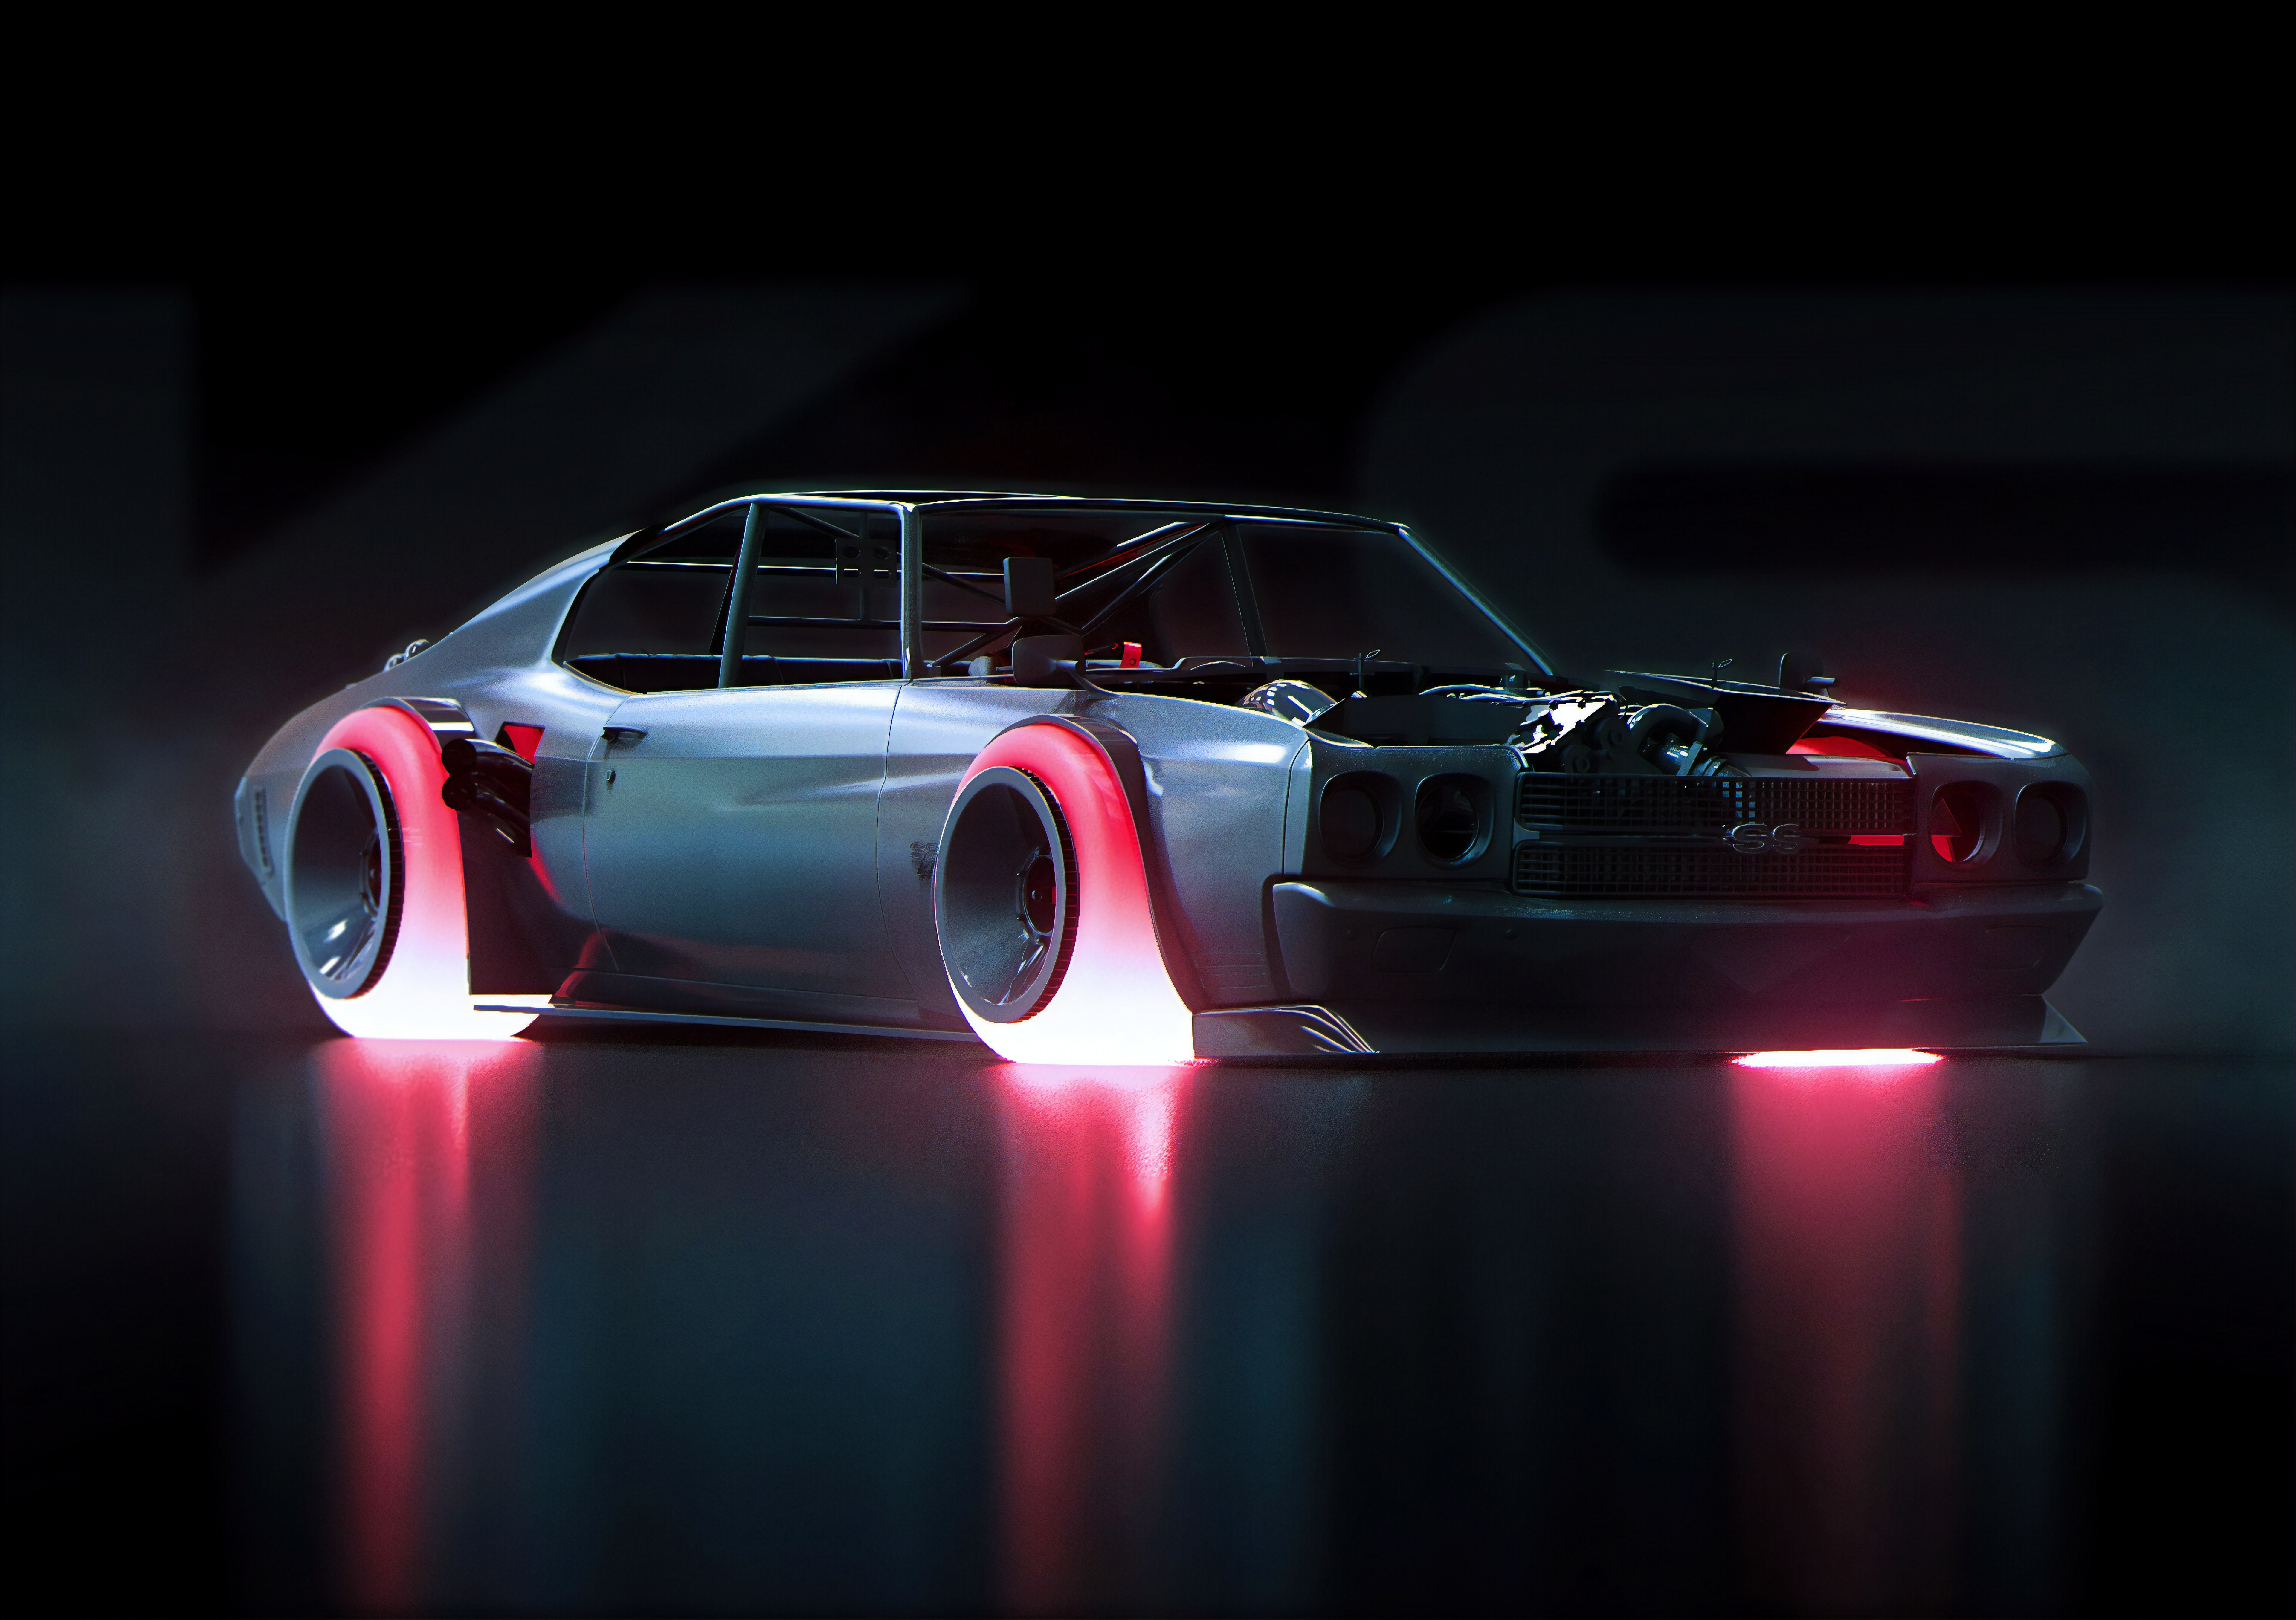
\includegraphics[width=\textwidth]{7.png}
			\caption*{仿真波形1}
		\end{minipage}
		\qquad
		\begin{minipage}{0.28\textwidth}
			\centering
			
\includegraphics[width=\textwidth]{8.png}
			\caption*{仿真波形2}
		\end{minipage}
		\\
		\begin{minipage}{0.28\textwidth}
			\centering
			\includegraphics[width=\textwidth]{7-1.png}
			\caption*{仿真结果}
		\end{minipage}
		\qquad
		\begin{tabular}{|c|c|c|c|}
			\hline
			& $U_o(mV)$ & $U_L(mV)$ & $R_o=(U_o/U_L)-1 \times R_L$ \\
			\hline
			仿真 & 998 & 949 & 51.633 \\
			\hline
			实验 & \quad & \quad & \qquad  \\
			\hline
		\end{tabular}
		\caption*{表4-3}
	\end{figure}
	\newpage
	\section*{四、测量放大器输入电阻}
	\begin{figure}[h]
		\centering
		
		\caption*{表4-2 }
	\end{figure}
	\begin{figure}[h]
		\centering
		\includegraphics[width=0.8\textwidth]{10.png}
		\begin{tabular}{|c|c|c|c|}
			\hline
			& $V_A(V)$ & $U_B(V)$ & $R_i=V_B/(V_A-V_B) \times R$ \\
			\hline
			仿真 & 0.7076 & 0.44769 & 8.78k  \\
			\hline
			实验 & \quad & \quad & \qquad  \\
			\hline
		\end{tabular}
		\caption*{表4-2 }
	\end{figure}
	\section*{五、测射极跟随器特性并测量输出电压峰值}
	\begin{figure}[h]
		\begin{minipage}{0.3\textwidth}
			\begin{tabular}{|c|c|c|c|c|}
				\hline
				仿真 & 1 & 2 & 3 & 4 \\
				\hline
				$U_i$ & 100mV & 200mV & 500mV & 800mV  \\
				\hline
				$U_L$ & \quad & \quad & \qquad & \quad \\
				\hline
				$U_{opp}$ & \quad & \quad & \quad & \quad \\
				\hline
				$A_v$ & \quad & \quad & \quad & \quad \\
				\hline
			\end{tabular}
			\caption*{表4-3}
		\end{minipage}
		\hspace{4cm}
		\begin{minipage}{0.3\textwidth}
			\begin{tabular}{|c|c|c|c|c|}
				\hline
				实验 & 1 & 2 & 3 & 4 \\
				\hline
				$U_i$ & 100mV & 200mV & 500mV & 800mV  \\
				\hline
				$U_L$ & \quad & \quad & \qquad & \quad \\
				\hline
				$U_{opp}$ & \quad & \quad & \quad & \quad \\
				\hline
				$A_v$ & \quad & \quad & \quad & \quad \\
				\hline
			\end{tabular}
			\caption*{表4-3}
		\end{minipage}
	\end{figure}
	\begin{figure}[h]
		\centering
		\begin{minipage}{0.6\textwidth}
			\centering
			
\includegraphics[width=\textwidth]{11.png}
			\caption*{仿真电路图}
		\end{minipage}
	\end{figure}
	
\end{document}